\chapter{CUDA}

The problem this thesis aims to solve is implementing an algorithm that is able to provide a hierarchical clustering of very large datasets while retaining the reasonable computation time --- the time required to compute a magnitude smaller datasets with current HCA algorithms.
Trying to achive this performance, we used a combination of C++ programming language and \emph{CUDA}\footnote{Compute Unified Device Architecture} API.

CUDA is a parallel platform and API allowing a programmer to use GPU for general purpose programming. This API exposes a computational power of~hundreds (even thousands) cores of CUDA-enabled GPUs~\cite{cuda}.


\section{Terminology}

The starting point for running any code on GPU using CUDA is a \emph{kernel}. A~kernel is a function that is executed on GPU; we say it contains \emph{device code}. Complementary to a device code, a \emph{host code} is the phrase for code executed on a CPU. Hence, a common CUDA application runs host code that determines which device code to run next. 

Kernel is run $n$ times in parallel by $n$ threads each having its unique \emph{thread ID}. IDs of threads can be identified by \emph{one-dimensional}, \emph{two-dimensional} or \emph{three-dimensional} indices forming block of threads, called \emph{thread block}. This property reflects shapes of common structures such as vectors and matrices resulting in~more natural computation.

Since all block threads reside on the same processor and share common resources, the block size is limited\footnote{Currently up to 1024 threads}. However, a kernel can be launched with multiple equally shaped blocks to increase the number of running threads. They can be organised into up to three-dimensional structure called \emph{grid}. This naturally implies unique block ID. A grid can be of an arbitrary size; usually dictated by~the~computed data (see fig.~\ref{fig02:grid}). It is a common practise that grid size surpasses the number of GPU processors.


\begin{figure}\centering
	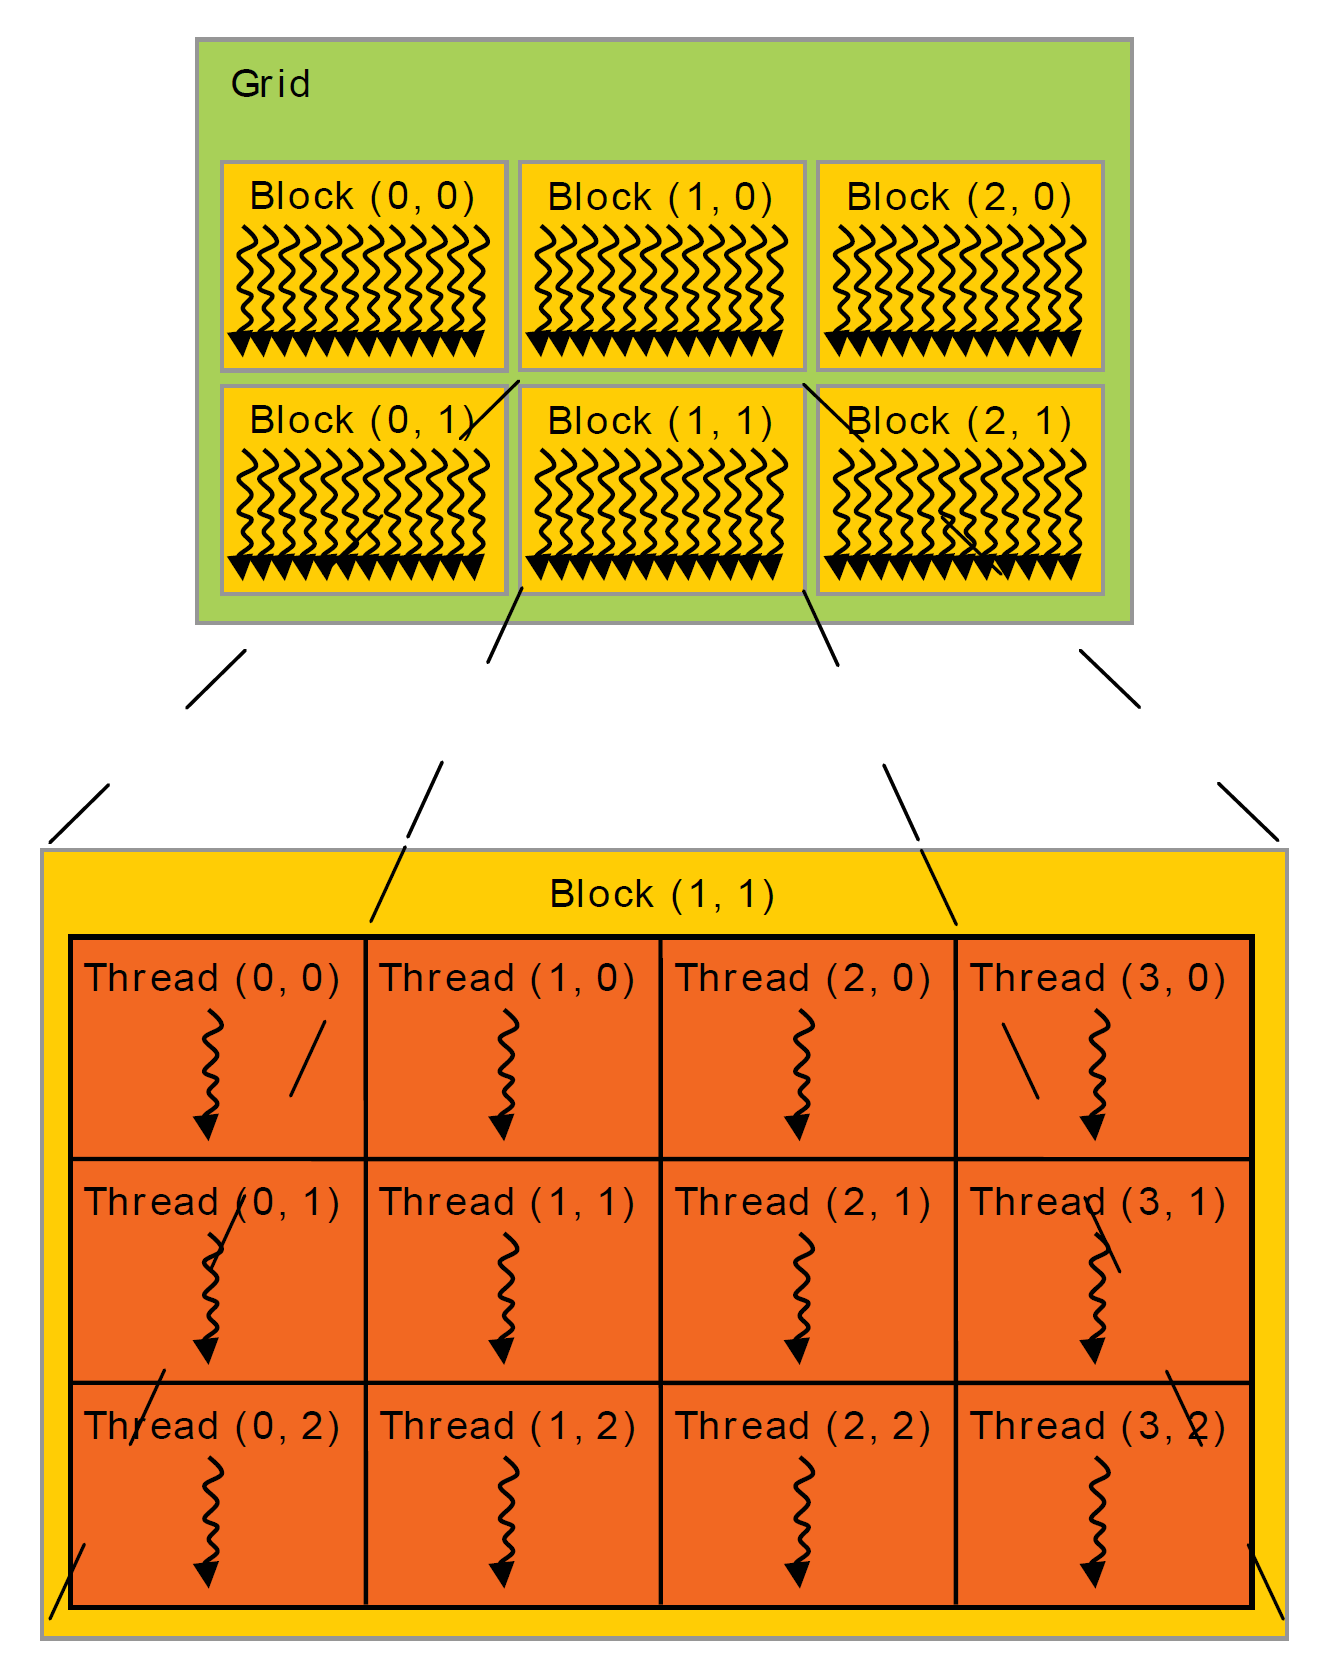
\includegraphics[width=7cm]{img/grid}
	\caption{An example of 2D grid of 2D size (3,2) with 2D blocks of 2D size (4,3).}
	\label{fig02:grid}
\end{figure}


The device memory is hierarchically divided into parts each being accessible by a different set of threads:

\begin{description}
	\item[Global memory] -- This memory is accessible by any thread. Any memory request is transferred via transactions; hence, to avoid decrease of the data throughput, memory accesses should be coalesced. 
	\item[Local memory] -- Each thread has exclusive access to its local memory. As it resides in a global memory, the local memory is a thread private global memory.
	\item[Shared memory] -- The shared memory is assigned to a block. It means that threads from the same block has access to the same shared memory. It is placed on-chip so it has much lower latency and higher bandwidth than the global or local memory.
	\item[Constant memory] -- The constant memory is a read-only memory accessible by any thread. Due to its read-only property, it can be heavily cached and may perform better than global memory. Together with global memory, it persists across different kernel launches.
\end{description}

The building block of the CUDA-enabled GPU hardware architecture is multi-threaded \emph{streaming multiprocessor (SM)}. A GPU contains an array of multiprocessors whose number varies between different GPUs. When a kernel launches, its grid of blocks is distributed among available multiprocessors and execute in parallel (see fig.~\ref{fig02:SM}). On the selected multiprocessor, block threads are executed in~parallel as well. Moreover, multiple blocks can run concurrently on one multiprocessor.

\begin{figure}\centering
 	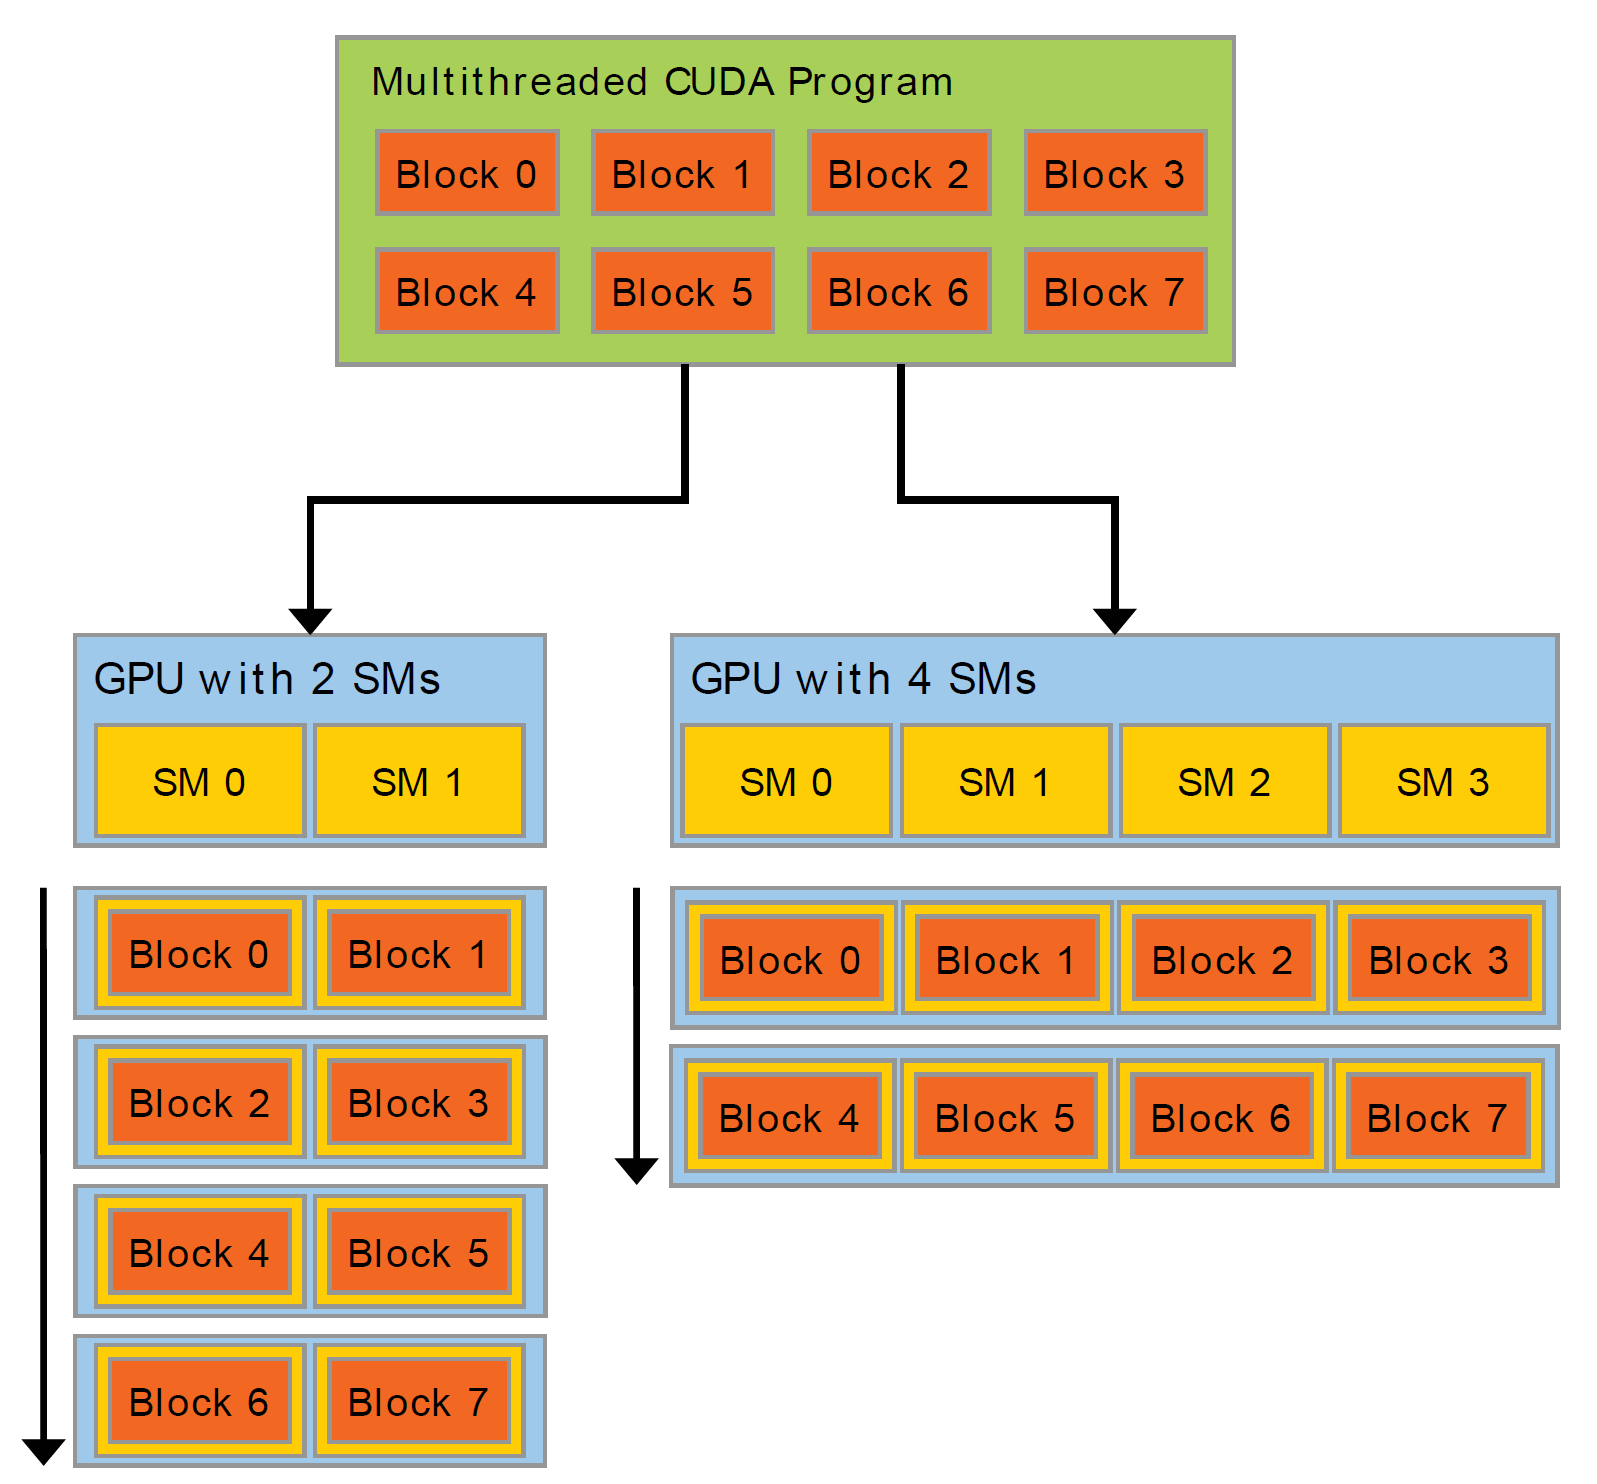
\includegraphics[width=8cm]{img/SM}
 	\caption{An example of different grid block distributions among SMs.}
 	\label{fig02:SM}
\end{figure}

To achieve this grade of parallelism, a GPU employs \emph{SIMT architecture} (Single Instruction - Multiple Threads). A~multiprocessor partitions an assigned block to chunks of 32 threads called \emph{warps}. Each warp thread is executed concurrently. During the execution, threads start with the the same program address but have own registers and instruction pointers so they can branch independently. However, a warp executes one common instruction at the time. Hence, to achieve the greatest performance all warp threads must agree on the program path.

Moreover, as warp threads execute concurrently, warp offers \emph{shuffle instructions}. All threads in warp are able to distribute their data to another thread within just one instruction. This comes to a great use for synchronization but can also be used to achieve high throughput reduction operations as well.
